% Options for packages loaded elsewhere
\PassOptionsToPackage{unicode}{hyperref}
\PassOptionsToPackage{hyphens}{url}
\PassOptionsToPackage{dvipsnames,svgnames,x11names}{xcolor}
%
\documentclass[
]{ccr}

% [WvA] change from original template.tex - amssymb is replaced by / clashes with newtxmath]
% \usepackage{amsmath,amssymb}
\usepackage{amsmath}

\usepackage{iftex}
\ifPDFTeX
  \usepackage[T1]{fontenc}
  \usepackage[utf8]{inputenc}
  \usepackage{textcomp} % provide euro and other symbols
\else % if luatex or xetex
  % [WvA] change from original template.tex - unicode-math is replaced by / clashes with newtxmath]
  %% \usepackage{unicode-math}
  \defaultfontfeatures{Scale=MatchLowercase}
  \defaultfontfeatures[\rmfamily]{Ligatures=TeX,Scale=1}
\fi
% Use upquote if available, for straight quotes in verbatim environments
\IfFileExists{upquote.sty}{\usepackage{upquote}}{}
\IfFileExists{microtype.sty}{% use microtype if available
  \usepackage[]{microtype}
  \UseMicrotypeSet[protrusion]{basicmath} % disable protrusion for tt fonts
}{}
\makeatletter
\@ifundefined{KOMAClassName}{% if non-KOMA class
  \IfFileExists{parskip.sty}{%
    \usepackage{parskip}
  }{% else
    \setlength{\parindent}{0pt}
    \setlength{\parskip}{6pt plus 2pt minus 1pt}}
}{% if KOMA class
  \KOMAoptions{parskip=half}}
\makeatother
\usepackage{xcolor}
\setlength{\emergencystretch}{3em} % prevent overfull lines
\setcounter{secnumdepth}{-\maxdimen} % remove section numbering
% Make \paragraph and \subparagraph free-standing
\ifx\paragraph\undefined\else
  \let\oldparagraph\paragraph
  \renewcommand{\paragraph}[1]{\oldparagraph{#1}\mbox{}}
\fi
\ifx\subparagraph\undefined\else
  \let\oldsubparagraph\subparagraph
  \renewcommand{\subparagraph}[1]{\oldsubparagraph{#1}\mbox{}}
\fi


\providecommand{\tightlist}{%
  \setlength{\itemsep}{0pt}\setlength{\parskip}{0pt}}\usepackage{longtable,booktabs,array}
\usepackage{calc} % for calculating minipage widths
% Correct order of tables after \paragraph or \subparagraph
\usepackage{etoolbox}
\makeatletter
\patchcmd\longtable{\par}{\if@noskipsec\mbox{}\fi\par}{}{}
\makeatother
% Allow footnotes in longtable head/foot
\IfFileExists{footnotehyper.sty}{\usepackage{footnotehyper}}{\usepackage{footnote}}
\makesavenoteenv{longtable}
\usepackage{graphicx}
\makeatletter
\def\maxwidth{\ifdim\Gin@nat@width>\linewidth\linewidth\else\Gin@nat@width\fi}
\def\maxheight{\ifdim\Gin@nat@height>\textheight\textheight\else\Gin@nat@height\fi}
\makeatother
% Scale images if necessary, so that they will not overflow the page
% margins by default, and it is still possible to overwrite the defaults
% using explicit options in \includegraphics[width, height, ...]{}
\setkeys{Gin}{width=\maxwidth,height=\maxheight,keepaspectratio}
% Set default figure placement to htbp
\makeatletter
\def\fps@figure{htbp}
\makeatother
\newlength{\cslhangindent}
\setlength{\cslhangindent}{1.5em}
\newlength{\csllabelwidth}
\setlength{\csllabelwidth}{3em}
\newlength{\cslentryspacingunit} % times entry-spacing
\setlength{\cslentryspacingunit}{\parskip}
\newenvironment{CSLReferences}[2] % #1 hanging-ident, #2 entry spacing
 {% don't indent paragraphs
  \setlength{\parindent}{0pt}
  % turn on hanging indent if param 1 is 1
  \ifodd #1
  \let\oldpar\par
  \def\par{\hangindent=\cslhangindent\oldpar}
  \fi
  % set entry spacing
  \setlength{\parskip}{#2\cslentryspacingunit}
 }%
 {}
\usepackage{calc}
\newcommand{\CSLBlock}[1]{#1\hfill\break}
\newcommand{\CSLLeftMargin}[1]{\parbox[t]{\csllabelwidth}{#1}}
\newcommand{\CSLRightInline}[1]{\parbox[t]{\linewidth - \csllabelwidth}{#1}\break}
\newcommand{\CSLIndent}[1]{\hspace{\cslhangindent}#1}

\makeatletter
\makeatother
\makeatletter
\makeatother
\makeatletter
\@ifpackageloaded{caption}{}{\usepackage{caption}}
\AtBeginDocument{%
\ifdefined\contentsname
  \renewcommand*\contentsname{Table of contents}
\else
  \newcommand\contentsname{Table of contents}
\fi
\ifdefined\listfigurename
  \renewcommand*\listfigurename{List of Figures}
\else
  \newcommand\listfigurename{List of Figures}
\fi
\ifdefined\listtablename
  \renewcommand*\listtablename{List of Tables}
\else
  \newcommand\listtablename{List of Tables}
\fi
\ifdefined\figurename
  \renewcommand*\figurename{Figure}
\else
  \newcommand\figurename{Figure}
\fi
\ifdefined\tablename
  \renewcommand*\tablename{Table}
\else
  \newcommand\tablename{Table}
\fi
}
\@ifpackageloaded{float}{}{\usepackage{float}}
\floatstyle{ruled}
\@ifundefined{c@chapter}{\newfloat{codelisting}{h}{lop}}{\newfloat{codelisting}{h}{lop}[chapter]}
\floatname{codelisting}{Listing}
\newcommand*\listoflistings{\listof{codelisting}{List of Listings}}
\makeatother
\makeatletter
\@ifpackageloaded{caption}{}{\usepackage{caption}}
\@ifpackageloaded{subcaption}{}{\usepackage{subcaption}}
\makeatother
\makeatletter
\@ifpackageloaded{tcolorbox}{}{\usepackage[skins,breakable]{tcolorbox}}
\makeatother
\makeatletter
\@ifundefined{shadecolor}{\definecolor{shadecolor}{rgb}{.97, .97, .97}}
\makeatother
\makeatletter
\makeatother
\makeatletter
\makeatother
\ifLuaTeX
  \usepackage{selnolig}  % disable illegal ligatures
\fi
\IfFileExists{bookmark.sty}{\usepackage{bookmark}}{\usepackage{hyperref}}
\IfFileExists{xurl.sty}{\usepackage{xurl}}{} % add URL line breaks if available
\urlstyle{same} % disable monospaced font for URLs
\hypersetup{
  pdftitle={Is Matilda Playing it Safe? Gender in Computational Text Analysis Methods},
  pdfauthor={Mariken A.C.G. van der Velden*; Alona O. Dolinsky},
  pdfkeywords={Computational Text Analyses Methods, Gender, Expert
Survey},
  colorlinks=true,
  linkcolor={blue},
  filecolor={Maroon},
  citecolor={Blue},
  urlcolor={Blue},
  pdfcreator={LaTeX via pandoc}}

\title{Is Matilda Playing it Safe? Gender in Computational Text Analysis
Methods}
\authorsnames{Mariken A.C.G. van der Velden*, Alona O. Dolinsky}
\authorsaffiliations{
    {Dept. of Communication Science, Vrije Universiteit Amsterdam}, 
    {Dept. of Communication Science, Vrije Universiteit Amsterdam}
}


\begin{document}
\abstract{Numerous studies document the gender gap in published articles
in political science journals, observing systematic imbalances in the
submission pool which result in a distored publication pattern. In this
study we test some pathways that may explain the distorted submission
pool: a) playing it safe due to the gender perception gap, and b) as a
consequence of the Matilda effect setting a higher bar for
methodological knowledge, focusing on papers using Computational Text
Analysis methods. Papers using Computational Text Analysis Methods are
more likely to be published in journals with a `masculinized' perception
gap. When women are aiming for these journals, they might `play it safe'
by conducting more validation checks than their male colleagues.
Moreover, embracing the Matilda effect -- i.e.~internalizing the
systematic under-recognition of female scientists and mis-attribution
of, especially methodological skills, to men -- women scholars are more
likely to indicate that a) there are important training needs in more
areas; and b) they themselves need (further) training in computational
methods and use these reasons not to publish papers employing these
methods. We test these claims using a) a unique content analysis of
research articles published in the top 20 journals in communication
science, political science, sociology and psychology between 2016 and
2020, identifying all 854 articles that involved some form of
quantitative textual analysis; and b) a pre-registered expert survey of
all authors of quantitative text analytic research identified via said
content analysis, which inquired about researchers' considerations and
concerns in the application of computational text analytic strategies.}
\keywords{Computational Text Analyses Methods, Gender, Expert Survey}
\maketitle
\volume{1}
\pubnumber{1}
\pubyear{2019}
\firstpage{1}
\doi{10.5117/CCR2019.1.001.VANA}
\shortauthors{van der Velden \&
Dolinsky}\ifdefined\Shaded\renewenvironment{Shaded}{\begin{tcolorbox}[sharp corners, boxrule=0pt, interior hidden, enhanced, frame hidden, borderline west={3pt}{0pt}{shadecolor}, breakable]}{\end{tcolorbox}}\fi

\hypertarget{introduction}{%
\section{Introduction}\label{introduction}}

The gender gap in the sciences and the social sciences has been debated
for decades (Hengel 2017; Huang et al. 2020; Monroe et al. 2008; Welborn
and McKenzie 1989). Numerous studies have documented gender disparities
in multiple areas of academia. These include publications and citations
of both journal articles and books (Young 1995; Teele and Thelen 2017;
Samuels and Teele 2021; Ferber and Brün 2011), collaborative projects
and co-authorships (Evans and Moulder 2011; König and Ropers 2018),
teaching evaluations (MacNell, Driscoll, and Hunt 2015; Mengel,
Sauermann, and Zölitz 2018), letters of recommendation (Madera et al.
2019), networking, socialization and mentorship (Barnes and Beaulieu
2017; Alter et al. 2020; Sarkees and Breuning 2010), evaluations of work
quality (Knobloch-Westerwick and Glynn 2013), promotion rates (Maliniak
et al. 2008; Key and Sumner 2019; Kim and Grofman 2019), status
recognition (Alter et al. 2020; Tatalovich and Frendreis 2019), grant
awards (Ma et al. 2019; Oliveira et al. 2019) and more. Despite efforts
to address these issues and the establishment of dedicated task forces
by academic organizations, such gender disparities persist across
disciplines (Alter et al. 2020; Dion, Sumner, and Mitchell 2018; Teele
and Thelen 2017; Weisshaar 2017). For example, the American Political
Science Association's Task Force on Systematic Inequalities in the
Discipline published a comprehensive report on January 2022 on the
multiple challenges affecting women in the field, discussing many of the
above areas of disparity.\footnote{The full report is available here:
  \url{https://connect.apsanet.org/sidtaskforce/}}

Among the various challenges affecting women in the discipline, of
particular importance is the gender gap in publication of academic work.
Publications are a key element of the profession, serving as both a
means to disseminate knowledge and as a metric by which productivity and
accomplishments are measured. This metric is then used as a basis for
promotion and advancement in the field, making it central for the
development of a successful career in academia. Thus, the gender gap in
publication of academic work has been the focus of numerous studies over
the years, examining a variety of possible explanations for the observed
skewed pattern (Breuning et al. 2018; Brown and Samuels 2018; Djupe,
Smith, and Sokhey 2019; Hill and Hurley 2022; König and Ropers 2018;
Teele and Thelen 2017). Among the various findings in these studies, a
common suggestion is that the gender gap in publications can be
explained by a distorted submission pool---men publish more papers
``simply'' because they submit more manuscripts. But why is the
submission pool distorted by gender? Some suggest that this is due to
skewed employment patterns, women scholars more likely to be employed at
teaching-focused institutions (Breuning et al. 2018), or due to other
factors like area of study or employed methodology (Hancock, Baum, and
Breuning 2013; Key and Sumner 2019). Others suggest a perception gap
affecting submissions-some journals are viewed as more ``masculinized'',
resulting in men being more likely to submit their work for
consideration at these journals compared to women (Brown et al. 2020).
Others still speculate that the gender gap in submissions results from
differences in quality standards and self-assessment (Brown et al. 2020;
König and Ropers 2018) as well as differences in taught publication
strategies through skewed socialization experiences (Brown et al. 2020).

Focusing on the study area of Computational Text Analysis Methods
(CTAM), which has grown significantly in the social sciences in recent
years, we test two possible pathways that may explain the distort
submission pool: a) playing it safe due to the gender perception gap,
and b) as a consequence of the Matilda effect setting a higher bar for
methodological knowledge. Papers using CTAM are more likely to be
published in journals with a `masculinized' perception gap. When women
are aiming for these journals, they might `play it safe' by conducting
more validation checks than their male colleagues. Moreover, embracing
the Matilda effect -- i.e.~internalizing the systematic
under-recognition of female scientists and mis-attribution of,
especially methodological skills, to men -- women scholars are more
likely to indicate that a) there are important training needs in more
areas; and b) they themselves need (further) training in computational
methods and use these reasons not to publish papers employing these
methods. In this paper, we are not testing the Matilda effect directly,
but we are investigating the consequences in scientific practices due to
the long-standing under-recognition of women scholars as well as the
active mis-attribution of their skills. We argue that the
internalization of this Matilda effect can be observed in wanting more
training or time, as this is an observable outcome of other forms of
academic socialization that create gender patterns, such as in
confidence, risk-taking, and self-valuation. We test these claims using
a) a unique content analysis of research articles published in the top
20 journals in communication science, political science, sociology and
psychology between 2016 and 2020, identifying all 854 articles that
involved some form of quantitative textual analysis; and b) a
pre-registered expert survey of all authors of quantitative text
analytic research identified via said content analysis, which inquired
about researchers' considerations and concerns in the application of
computational text analytic strategies.\footnote{Replication files are
  available on the
  \href{https://github.com/MarikenvdVelden/gender-ctam}{corresponding
  author's Github account}}

Examining authors' gender distribution among the 854 articles using
quantitative textual analysis shows a significant gender gap especially
in CTAM studies which were authored by 501 male scholars compared to
only 209 female scholars. These patterns underlay the importance of an
introspective evaluation of what might explain this observed gender gap.
Examining the survey data, our findings are slightly optimistic: In
social science disciplines where CTAM has become more prevalent, women
scholars catch up quickly and we do not see a ``play it safe'' strategy:
Women do not report to conduct much more validation checks when using
computational text analyses methods. We do see, however, that in
disciplines where CTAM is less of a mainstream method, this strategy is
in place. At the same, our findings show various indications of the
internalization of the Matilda effect, i.e.~the consequences thereof, at
play: Women scholars perceive that a lot more effort is required for
women to succeed in the profession. This has important downstream
consequences for women scholars in their careers: Lower output,
out-selecting of grant proposals and team work. To this end, it is
important that infrastructure of both training and data acknowledges
these gender disparities as well as actively take action, as we see that
especially the playing it safe mechanism can be alleviated. This in turn
potentially mitigates the influence of the Matilda effect as well.

\hypertarget{gender-distortion-in-the-submission-pools-a-matter-of-playing-it-safe}{%
\section{Gender distortion in the submission pools: A matter of playing
it
safe?}\label{gender-distortion-in-the-submission-pools-a-matter-of-playing-it-safe}}

Numerous studies have examined the gender gap in academic publications,
finding both positive and negative associations with various proposed
explanations. Breuning et al. (2018), for example, found no supporting
evidence for the proposition that women scholars publish less than their
male colleagues because of differences in areas of study. Similarly,
König and Ropers (2018) did not find support for the proposition that
women scholars publish less than their male colleagues because of
differences in used research methods, although Teele and Thelen (2017)
and Brown and Samuels (2018) did observe such a pattern. Further still,
König and Ropers (2018) and Djupe, Smith, and Sokhey (2019) found no
evidence that work by women is rejected more frequently than that of men
relative to their submission rates, and Breuning et al. (2018), König
and Ropers (2018), and Brown and Samuels (2018) found no evidence of a
gender bias in the editorial process itself. While these explanations
can seemingly be ruled out as causes of the gender gap in publications,
other explanations do find support. Breuning et al. (2018), for example,
found evidence that journal editors exhibit a preference for authors in
research-intensive universities, indicating that while some bias exists
in the editorial process itself, it is not explicitly gender-based. The
most notable finding across these studies is a common suggestion that
fundamentally, the gender gap in publications can be explained by a
distorted submission pool---that men publish more papers ``simply''
because they submit more manuscripts (König and Ropers 2018; Brown and
Samuels 2018; Breuning et al. 2018).

So what might explain the gender distortion in the submission pools? Few
studies offer systematic evidence with which to answer this question,
but the literature does offer several speculative explanations. Breuning
et al. (2018), for example, speculate that women scholars submit fewer
manuscripts for review because they are more likely to be employed at
teaching-focused institutions where less value is put on publications.
Other studies point to a perception gap affecting submission rates.
Brown et al. (2020), for example, argue that some journals, like
American Political Science Review, American Journal of Political
Science, and Political Analysis are perceived to be ``masculinized''
with men significantly more likely than women to state that they would
submit their manuscripts to these journals. Moreover, men are more
likely than women to be optimistic about their chances of successful
publication in these journals, a perception that is maintained even when
controlling for scholars' methodological approach. Hancock, Baum, and
Breuning (2013) (in International Studies) and Key and Sumner (2019)
suggest that differences in area of study and/or applied methodology
explain the gender gap in submissions, while Djupe, Smith, and Sokhey
(2019) find that the gender gap persists within methodological
approaches---women who state that their work is primarily
quantitative-statistical submit fewer papers for review than their male
colleagues. Brown et al. (2020) further speculate that women are also
more risk averse than men and are therefore less willing to submit their
work to journals with high rejection rates (see Djupe, Smith, and Sokhey
(2019) and Key and Sumner (2019) for similar arguments). Djupe, Smith,
and Sokhey (2019) also find that male assistant professors ``flood'' the
review process with submissions and receive a higher number of
rejections, while König and Ropers (2018), finding a similar pattern,
speculate that this may suggest that ``male and female authors have
different quality standards when submitting their work in the first
place\ldots{}'' (p.~851). Brown et al. (2020) similarly argue in a
footnote that ``it also could be the case that women scholars are more
likely to underestimate the quality of their work and therefore are less
likely to submit\ldots{}'' (p.~120, fn 10). Adding to these debates, we
propose to look at a different explanation, one that is potentially of
large consequences when it comes to employing CTAM.

\hypertarget{the-matilda-effect-and-its-consequences}{%
\section{The Matilda Effect and its
Consequences}\label{the-matilda-effect-and-its-consequences}}

While it is difficult to determine the root cause of the gender
differences in self-perceptions of quality of work and the prospects of
successful publication that might lead to a gender submission gap, we
suggest that this may be related to the Matthew Effect and its mirror
the Matilda Effect. Made famous in the late 1960s by the American
sociologist Robert K. Merton, the Matthew Effect refers to the
over-recognition of scholars at the top of the scientific profession.
This over-recognition is rooted in a cycle wherein those who already
have (recognition) gain more of it, while those who have little, will
continue to have little. As men have historically been at the top of the
scientific profession, the ``trickle down'' influence of the Matthew
Effect can be observed in the gendered patterns discussed above. Thus,
while it may indeed be the case that the publication process and its
outcomes are not purposefully biased against women scholars, there is
nevertheless a systematic gender difference in academic publishing we
can trace that is linked to other gendered imbalances in the profession.
In particular, co-authored manuscripts are more likely to be published,
and the rise in co-authorship is primarily driven by all-male teams
(Teele and Thelen 2017). And, even if men and women are equally likely
to co-author (Djupe, Smith, and Sokhey 2019), male scholars benefit
significantly more from such collaborations in terms of both submissions
and publications. Why? Similar to their argument above about differences
in publication strategies due to differentiated socialization, Brown et
al. (2020, 119) speculate that ``something happens to men in their
collaborative networks that bolsters their likelihood to submit papers
and to resubmit previously rejected papers. Younger male scholars in
highly productive collaborative groups may be more likely to receive
encouragement for and to develop early habits of frequent article
submission. They also may feel more inoculated against the
morale-damaging effects of rejection from top-tier journals''.

What does it mean that men are more likely than women to collaborate and
therefore produce more work for publication? The flip side of this
argument is the observation from Brown and Samuels (2018, 329) that ``to
the extent that women are less likely to be invited onto a team or form
collaborations themselves (perhaps because mentors do not think to
encourage them to do so), they are less likely to expand their citation
networks, less likely to get cited, and less likely to rise through the
ranks\ldots{}''. This, in turn, can be linked we argue, to the mirror of
the Matthew Effect---the \emph{Matilda Effect}. Coined by Margaret W.
Rossiter in 1993, the Matilda Effect refers to the under-recognition of
women in the sciences and the social sciences as well as the the
phenomenon that women's work gets attributed to men (Rossiter 1993),
which persists across decades. For example, in the early 1990s, Cole and
Singer (1991) observed that while there is not much gender difference in
achievement levels at the early stages of academic careers, women's
careers trajectories are affected more by negative results than those of
men. Numerous studies also document gender distortions in citations
(Tatalovich and Frendreis 2019; Maliniak, Powers, and Walter 2013;
Samuels and Teele 2021; Dion, Sumner, and Mitchell 2018; Ferber and Brün
2011); promotion (Key and Sumner 2019; Kim and Grofman 2019; Maliniak et
al. 2008) and visibility on graduate syllabi (Phull, Ciflikli, and
Meibauer 2019; Colgan 2016). Tatalovich and Frendreis (2019) further
show that while women win more awards today than in the past, they are
still unable to match the scholarly recognition men receive for their
work.

The focus on and use of computational text analysis has grown
significantly in recent years and has taken a prominent place in the
study of political texts within the discipline (see for example: Lazer
et al. 2020; Salganik 2019). Within computational text analysis, and
quantitative research methodology in general, women are particularly
underrepresented, studies showing a gender gap across levels in these
fields. For example Gatto et al. (2020) found that women, on average,
cover significantly fewer methods courses in their graduate training
compared to their male colleagues, and that women are more likely than
men to complete qualitative methods courses. Barnes (2018) shows that
women are less likely to be lecturers in quantitative methods courses.
Furthermore, while Gatto et al. (2020) also found that when women do
participate in methods training they show similar levels of method
employment as their male colleagues, Shannon (2014) and Esarey (2018)
found that even when women do use the same methods as men, they are less
likely to characterize themselves as methodologists. This echoes
findings from Morrow-Jones and Box-Steffensmeier (2014) and Shannon
(2014) that women's self-evaluation of math-related qualifications tends
to be lower than men's, even when they outperform them. Still further,
Teele and Thelen (2017) and Brown and Samuels (2018) show that women are
less likely to publish studies using quantitative and computational
methods, Maliniak, Powers, and Walter (2013) making a similar argument
in International Relations studies.

\hypertarget{expectatations}{%
\section{Expectatations}\label{expectatations}}

Building on the last of these observations and focusing on social
science scholarship using computational text analysis methods, we
contribute to the debate about possible explanations for a gendered
submission gap by proposing two additional explanations: a) playing it
safe due to the gender perception gap of journals, and b) In this study
we test some pathways that may explain the distorted submission pool: a)
playing it safe due to the gender perception gap, and b) as a
consequence of the Matilda effect setting a higher bar for
methodological knowledge. Papers using CTAM are more likely to be
published in journals with a \emph{``masculinized'' perception gap}.
These are journals that ``men are significantly more likely than women
to state that they would submit a manuscript and/or be optimistic about
their chances of publication'' (Brown et al. 2020, 115). Moreover, given
that women may tend to also be more risk averse than men (Brown et al.
2020), when women are aiming for these journals, it could be that they
``play it safe'\,' by conducting more validation checks than their male
colleagues. Embracing the idea of the \emph{Matilda effect} --
internalizing that a lot more effort is required to women to succeed in
academia due to systematic under-recognition and mis-attribution --
women scholars are more likely to indicate that a) there are important
training needs in more areas; and b) they themselves need (further)
training in computational methods and use these reasons to not submit,
or submit less work that employs these methods. That is, as women
embrace the underlying notion of the Matilda Effect they perceive that
they need to work that much harder to prove themselves to be at the same
level as men in order to reach at par results. We examine the following
hypotheses:

\textbf{Play it Safe hypothesis} (\emph{H1a}): Women scholars are more
likely to play it safe and indicate more validation strategies than men
scholars.

\textbf{Play it Safe hypothesis} (\emph{H1b}): Women scholars are more
likely to play it safe and indicate more challenges as reasons
\textbf{not} to use CTAM than men scholars.

\textbf{Matilda effect hypothesis} (\emph{H2a}): Women scholars are more
likely to indicate a higher number of important training needs than men
scholars.

\textbf{Matilda effect hypothesis} (\emph{H2b}): Women scholars are more
likely to indicate that they themselves require (further advanced)
training than men scholars.

\hypertarget{data-measures}{%
\section{Data \& Measures}\label{data-measures}}

Building on a content analysis study of published articles conducted by
Baden et al. (2021), we conducted an expert survey, inviting all
scholars who had published a scientific article using quantitative text
analysis between January 2016 and September 2020 in one of the 20
highest ranked journals in Communications, Political Science, Sociology,
and Psychology (for more details, see Baden et al. 2021). Quantitative
textual analysis was defined broadly to include any form of processing
natural language that identified specific kinds of textual contents with
the purpose of classification and quantitative analysis. Using a keyword
search on the Web of Science, we identified a total of \texttt{7,296}
\emph{potentially} relevant articles out of the \texttt{45,437}
published articles, whose abstract suggested any kind of textual content
or test analytic procedures.\footnote{As discussed in Appendix A of
  Baden et al.~2021 on which our survey is built, the following keywords
  were used: ``SO=''{[}Journal{]}'' AND AB=(language* OR text* OR
  discours* OR coverag* OR speech* OR document* OR fram* NOT framework
  OR content* OR code* OR coding OR classif* OR ``big data'' OR
  ``machine learning'' OR ``dictionary'' OR ``SML'' OR ``topic model''.}
Articles were considered relevant as soon as they used any form of
quantitative textual analysis, even if it was used merely in an
auxiliary capacity (e.g., a content analysis to identify frames to be
used in an experiment; sentiment analyses of open-ended survey
responses).\footnote{Analyses that relied solely on metadata or
  pre-existing classification were excluded, as were investigations
  accessing only formal properties of the sampled texts (e.g., length).
  We included analyses of multi-modal media (e.g., posters, television)
  as long as the textual contents were informative toward
  classification. Purely methodological contributions discussing
  specific potentials or limitations of available methods were excluded,
  unless they included applied demonstrations wherein actual textual
  data were processed.} This keyword-based screening yielded a total of
\texttt{854} articles, for which the authors were looked up.\footnote{As
  Baden et al.~2021 note, those 854 articles show an increase in
  computational methods -- from 35 in 2016 to 79 in 2020 -- and the
  amount of manual content analysis stays the same (around 100 each
  year).} This gave us \texttt{1,653} identifiable and working
email-addresses. The experts were invited to the questionnaire on March
4th of 2021, and received two reminders, each approximately a week after
our last message (respectively on March 11th and March 16th of 2021).
This yielded a responses of \texttt{433} responses (i.e.~response rate
of \texttt{25\%}). Of these respondents, 142 were male scholars and 243
were female scholars.\footnote{The two respondents who identified with
  neither gender are left out of this study. For the full questionnaire
  see Appendix B in Baden et al.~2021 (https://osf.io/ev85x).} This
means that women were more likely to respond to the survey -- 56\% in
the sample of the survey, where they are only 39\% of the author
population. The study has been approved by the Research Ethics Review
Committee of the \protect\hyperlink{}{\emph{Vrije Universiteit
Amsterdam}}, \protect\hyperlink{}{\emph{Hebrew University Jerusalem
Isreal}}, and \protect\hyperlink{}{\emph{University College Dublin}}.

To motivate our claim of a gender gap in CTAM, we coded the first four
authors of the 854 articles, leading to 1,844 identifiable names. For
these names, we hand-coded the gender of the authors --- if pronouns
were not given, we assumed gender is equally to sex.\footnote{We could
  not use an automated approach, e.g.~like the gender R package, as
  quite some non-European names would not been assigned, leading to a
  bias in our sample.} We identified the author's gender because either
the author was known to us, and we therefore knew their gender or we
assumed gender based on the picture and if available references in the
author's bio (e.g.~his/her). The coding identified 1,133 male scholars
and 711 female scholars. Breaking this down by the use of CTAM or manual
content analysis methods (MTAM)\footnote{This distinction is based on
  the data coded by Baden et al.~2021.}, we see that MTAM are used by
respectively 502 and 632 female and male scholars, showing a small
gender difference. Among studies using CTAM, however, we find a
significant gender disparity, this method being used by respectively 209
and 501 female and male scholars. Furthermore, we compare the likelihood
of a male author being the first, second, and third author respectively
compared to a female author on that position via an independent T-test.
We do this for a) the whole sample of articles; b) the articles that use
CTAM; and c) the articles that use MTAM.

\begin{figure}[t]

{\centering 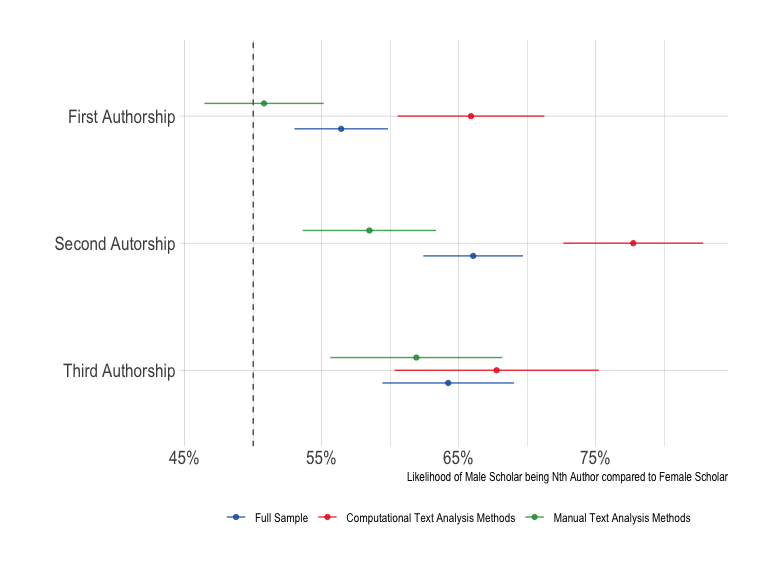
\includegraphics[width=1\textwidth,height=\textheight]{figures/ttest-1.png}

}

\caption{\label{fig:ttest}Gender Break-Down of Article Authorship}

\end{figure}

Figure \ref{fig:ttest} shows that men are more likely to be first author
in the entire sample. This effect is driven by first authorship in CTAM
articles, in which men are significantly more likely to be first authors
compared to females --- the same pattern holding for second and third
author. Figure \ref{fig:ttest} additionally shows that males are more
likely to be first and second author in CTAM articles compared to the
sample of articles of both CTAM and MTAM. These findings showcase the
existence of a gender gap in CTAM, reinforcing our motivation to examine
possible explanations for this observed gender gap.

\begin{figure}[t]

{\centering 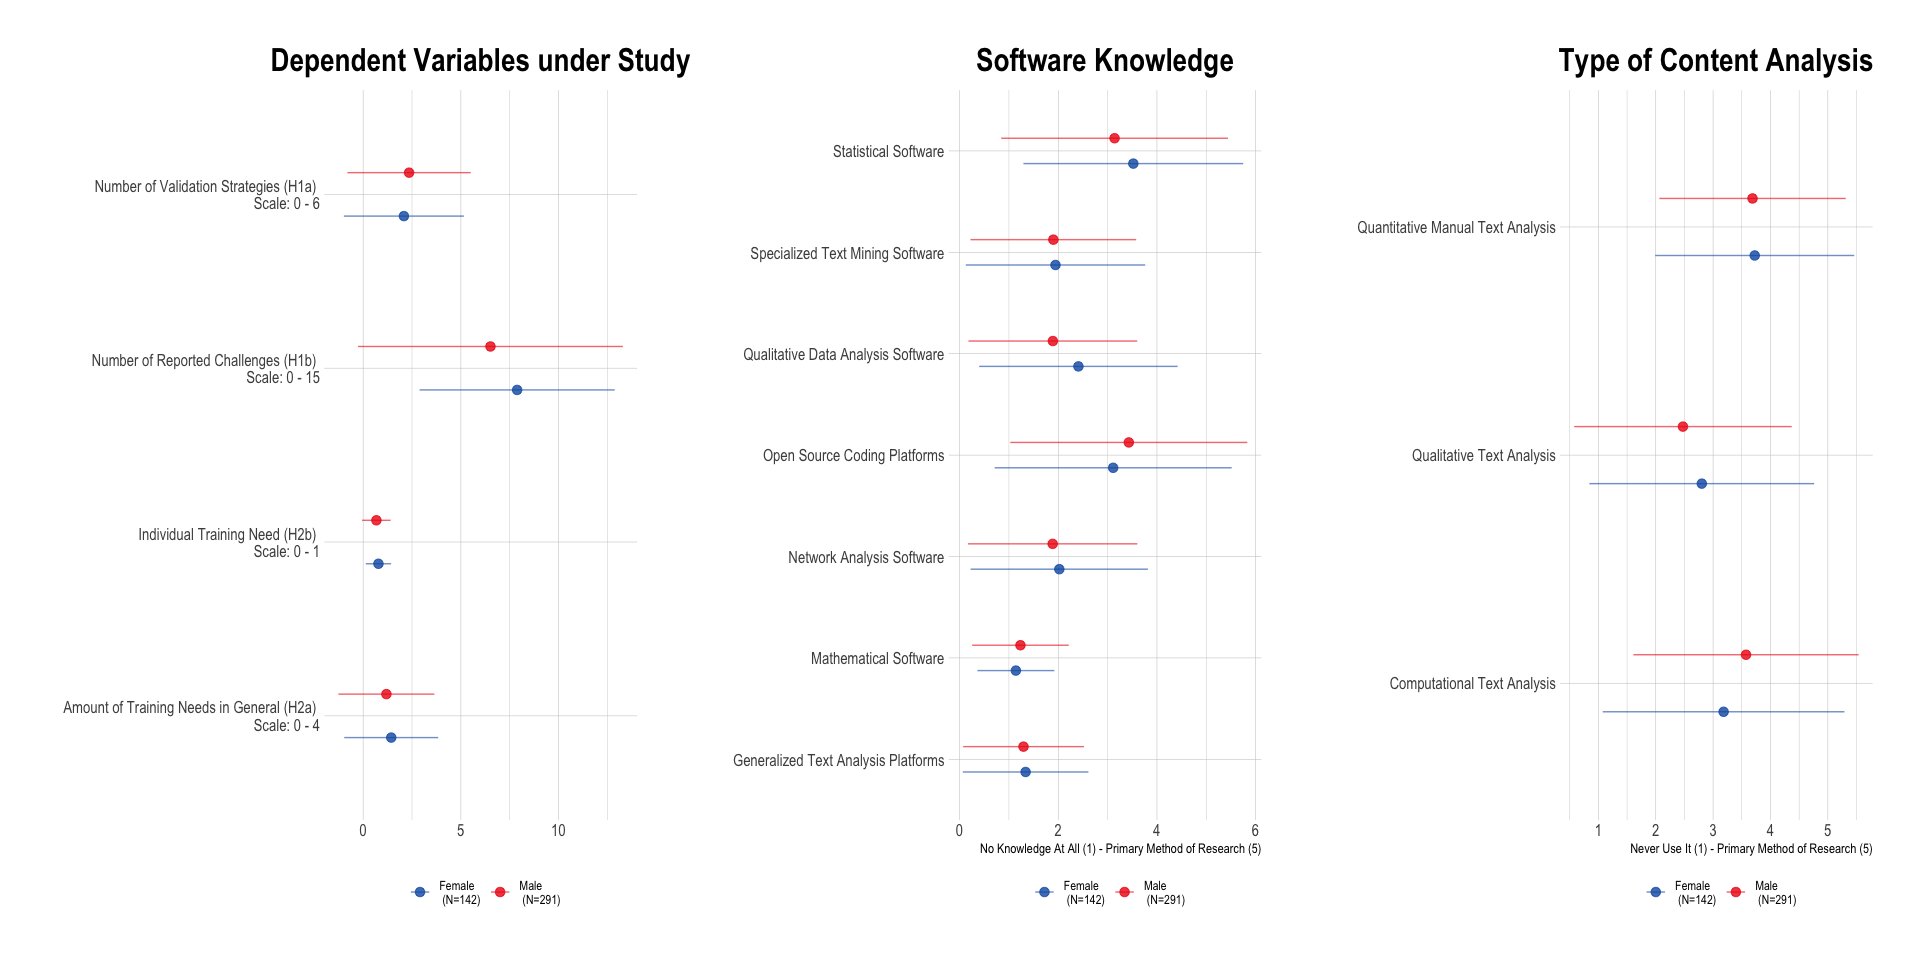
\includegraphics[width=1\textwidth,height=\textheight]{figures/explorative-1.png}

}

\caption{\label{fig:descr}Gender Break-Down in Variables under Study}

\end{figure}

To survey the field on different aspects of potential `playing it safe'
strategies when it comes to CTAM, we have asked participants to list how
many of five pre-defined validation strategies\footnote{The pre-defined
  validation strategies are: 1) \emph{I check the documentation of the
  software developer}; 2) \emph{I check whether findings are plausible
  and interpretable}; 3) \emph{I compare machine-made classifications
  (i.e.~coded outputs) against manually coded/given standards}; 4)
  \emph{I check whether the classification rules/criteria are valid
  (e.g., check for meaningful indicators in adictionary)}; and 5)
  \emph{I evalute how well the algorithmic procedures match my concept
  of interest (e.g., checking adequacy of bag-of-words assumption)}.}
they use, as well as if they use other strategies (open answer
possibility).\footnote{There are different strategies as to how someone
  can play it safe. The big difference of CTAM compared to MTAM is the
  amount of control the researcher has over the process. Where MTAM is
  determined by the researcher, e.g.~by making a codebook, and the
  validation thereof is formalized by a reliability test (Krippendorff
  2013), which is then used in full control of the author to process and
  analyse texts, the same is not case when CTAM are used. In the case of
  CTAM, the validation process is less clear for unsupervised methods,
  the standards are not quite set (Baden et al. 2021), and there is less
  control by the researcher to fully understand what the algorithm is
  doing. This makes it possible to fiddle around with alternatives until
  the measurement is ``good enough''.} Additionally, we asked
participants to what extent 15 pre-defined reasons were a relevant
challenge for them in deciding to \emph{not} to use CTAM.\footnote{The
  pre-defined challenges are: 1) \emph{Time/effort required
  (e.g.~technical requirements, experience)}; 2) \emph{Funding required
  (e.g., for training, fees)}; 3) \emph{Availability of required
  training in computational methods}; 4) \emph{Limited methodological
  guidance/documentation of tools}; 5) \emph{Level of instruction and
  materials higher than needed}; 6) \emph{Level of instruction/materials
  lower than needed}; 7) \emph{Availability of suitable computational
  tools for certain languages}; 8) \emph{Comparability of computational
  tools in different languages}; 9) \emph{Issues concerning measurement
  validity/limited nuance}; 10) \emph{Loss of manual contact with the
  material}; 11) \emph{Reviewers'/editors'\,' skepticism toward
  computational methods among}; 12) \emph{Peers' skepticism toward
  computational methods}; 13) \emph{I am skeptical toward computational
  methods myself}; and 14) \emph{Other challenges: (Open ended)}.}
Answer options where \texttt{no\ challenge}, \texttt{minor\ challenge},
\texttt{major\ challenge}. Examining whether there exists a gender gap
in the extent of reported challenged, we analyze whether women more than
men report major challenges compared to minor challenges controlled for
the other variables we use in the study as controls. As Figure
\ref{fig:challenge1} shows, female scholars are more likely to report
challenges as major compared to male scholars. Additional T-tests
confirm this as shown in Figure \ref{fig:challenge2}, where even the
average scores are statistically significant for the challenges: Time
required, Limited methodological guidance/documentation of tools, Level
of available instruction/materials higher than needed, Funding required,
Availability of suitable computational tools for specific measurement
purposes, and Availability of required training. This could be another
indication for women scholars either playing it safe or internalizing
the Matilda effect.

\begin{figure}[t]

{\centering 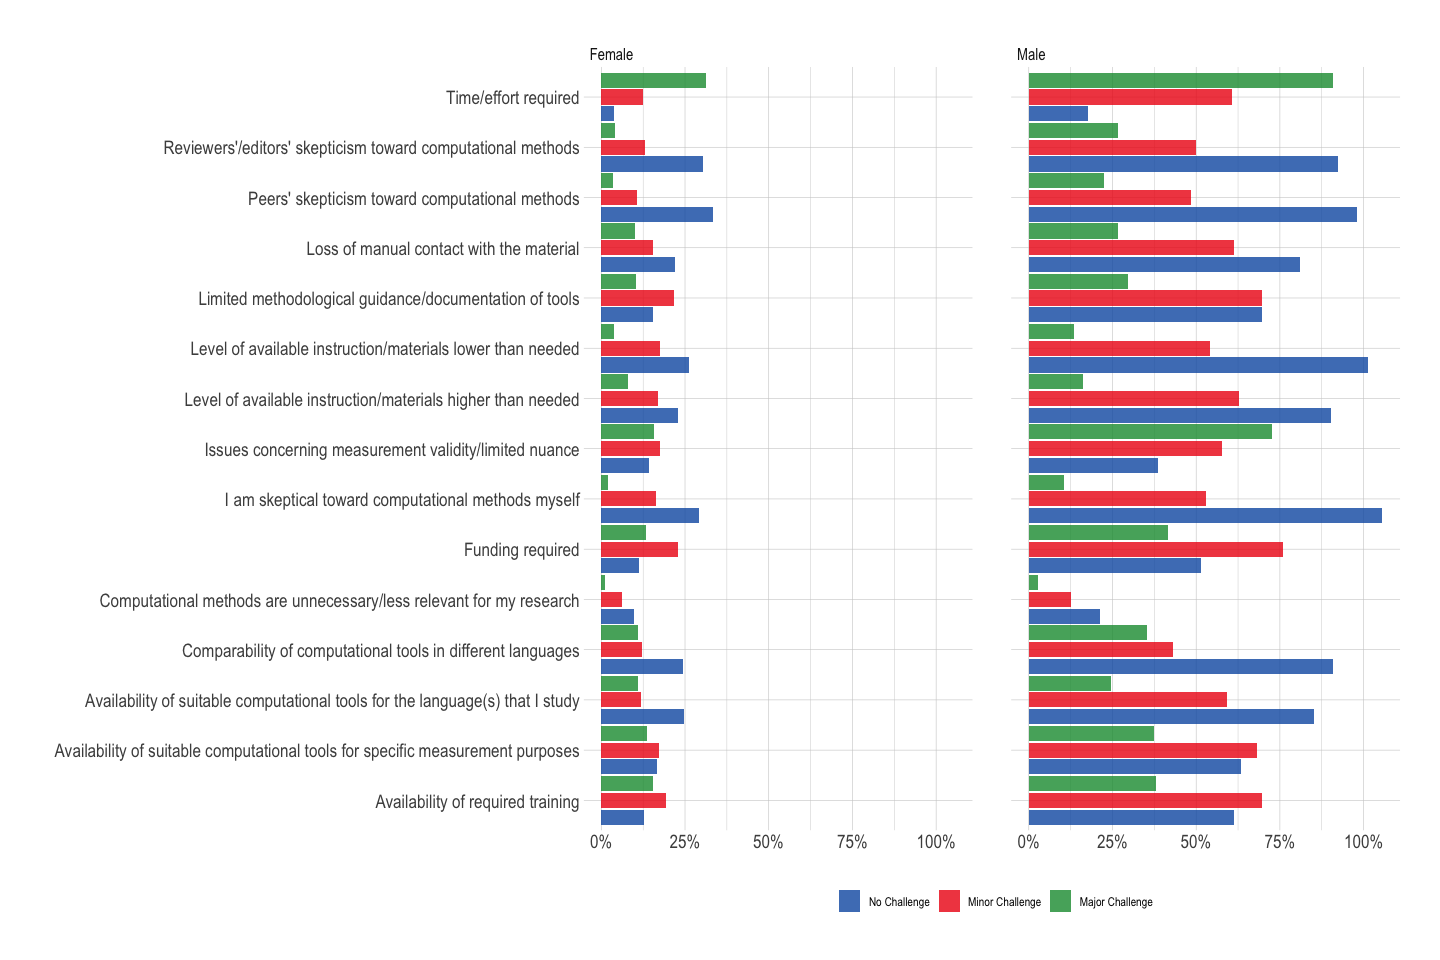
\includegraphics[width=1\textwidth,height=\textheight]{figures/challenges-distribution-1.png}

}

\caption{\label{fig:challenge1}Challenges relevant to scholars' decition
to not use CTAM}

\end{figure}

\begin{figure}[t]

{\centering 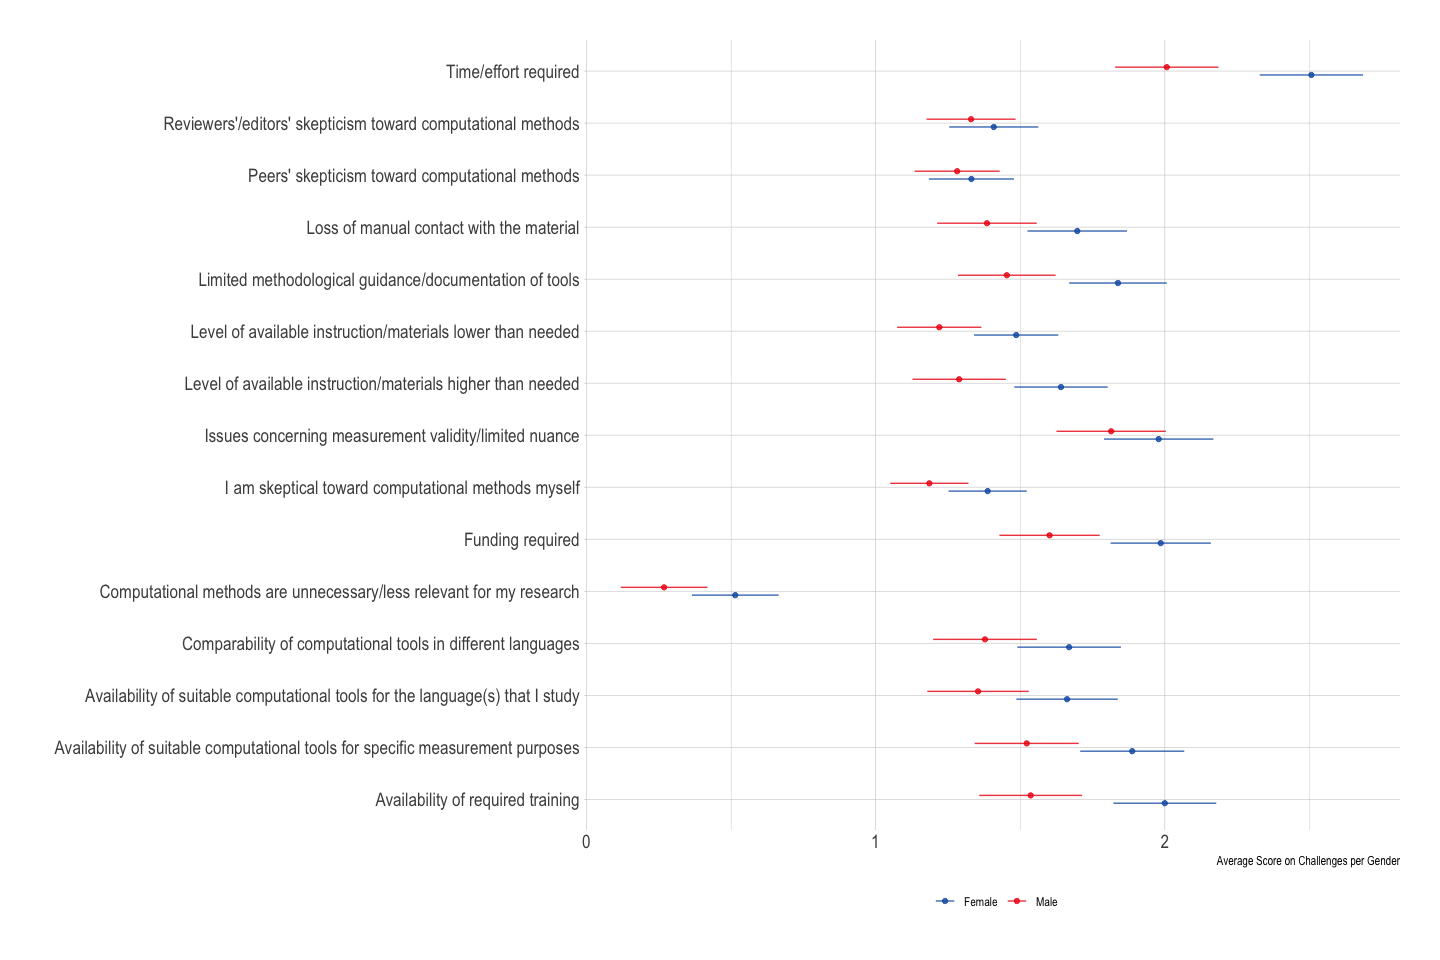
\includegraphics[width=1\textwidth,height=\textheight]{figures/challenges-distribution-2.png}

}

\caption{\label{fig:challenge2}Challenges relevant to scholars' decition
to not use CTAM}

\end{figure}

In the main analyses, we grouped minor and major challenges together and
compared them to no challenges reported. To gauge a possible influence
of the `Matilda effect', we asked our experts to list if the field in
general needs more training possibilities when it comes to data and open
access tools, programming and software skills, theory and concepts,
research integrity and ethics, or other training skills -- for each
option there was the possibility to specify what was needed. Moreover,
we also asked respondents if they themselves need more training. In all
our analyses, we control for whether or not the respondent uses CTAM
themselves, the types of content analyses they use in their work, and
their pre-existing knowledge of statistical software. Figure
\ref{fig:descr} shows the gender break-down in our sample for the
dependent variables as well as the control variables. While the
descriptive statistics (average and standard deviation) do not show
statistically significant gender differences, we do see in the top-right
panel that men in our sample are over-represented. Yet where we have
roughly the same amount of women scholars using CTAM as not using CTAM
(i.e.~using quantitative or qualitative manual content analysis), our
sample has more men scholars using CTAM than not using CTAM. Moreover,
the top-left panel shows that men report fewer challenges for uptaking
computational methods than women do.

\hypertarget{is-matilda-playing-it-safe}{%
\section{Is Matilda Playing it Safe?}\label{is-matilda-playing-it-safe}}

To test our pre-registered hypotheses, we ran a OLS regression and
visualize the results in Figure \ref{fig:pre-reg-h} and
\ref{fig:dv-types} with an one-tailed \(\alpha\) of \texttt{0.05}.
Looking at the variables measuring `playing it safe' strategies,
i.e.~reporting number of validation strategies and number of challenges,
Figure \ref{fig:pre-reg-h} demonstrates that women scholars do not
report more validation strategies than men. However, women that use
qualitative methods report to use less validation strategies. This can
potentially be explained by the fact that qualitative text analysis
involves fewer validation strategies. In the top-left panel of Figure
\ref{fig:dv-types}, we inspect the gender differences in the type of
validation strategies reported. This shows that the only strategy women
scholars are statistically significantly less likely to report compared
to men scholars is checking the documentation of the software developer.
In the Research Software Community, there is a recent uptake on
addressing inclusiveness to address this disparity (e.g.~see, Gruber and
Velden (2023)). Women scholars are more likely to report to use the
validation strategies of checking algorithmic procedures and checking
against the gold standard. This is only borderline non-significant, most
likely due to the small number of women in our sample. For the other
playing it safe strategy -- i.e.~number of challenges reported -- Figure
\ref{fig:pre-reg-h} shows that women scholars are more likely to report
challenges, but this effect is not statistically significant. Breaking
down the challenges, shown in the right-hand panel of Figure
\ref{fig:dv-types}, does demonstrate an interesting gender pattern.
Women are more likely to report time/effort, funding, and training needs
as well as limited methodological guidance of the tools as a challenge
to not using CTAM. Men scholars, however, are more taken back by peers'
and editors' skepticism towards the method (as also shown in
\ref{fig:challenge1} and \ref{fig:challenge2}). This is a mild
indication of the consequences of the Matilda Effect's influence at
play: Men, more likely to be confident of being recognized for their
work, place a higher premium on peer perception while women, taken in by
the Matilda Effect, think a lot more effort is required of them to be
successful.

\begin{figure}[H]

{\centering 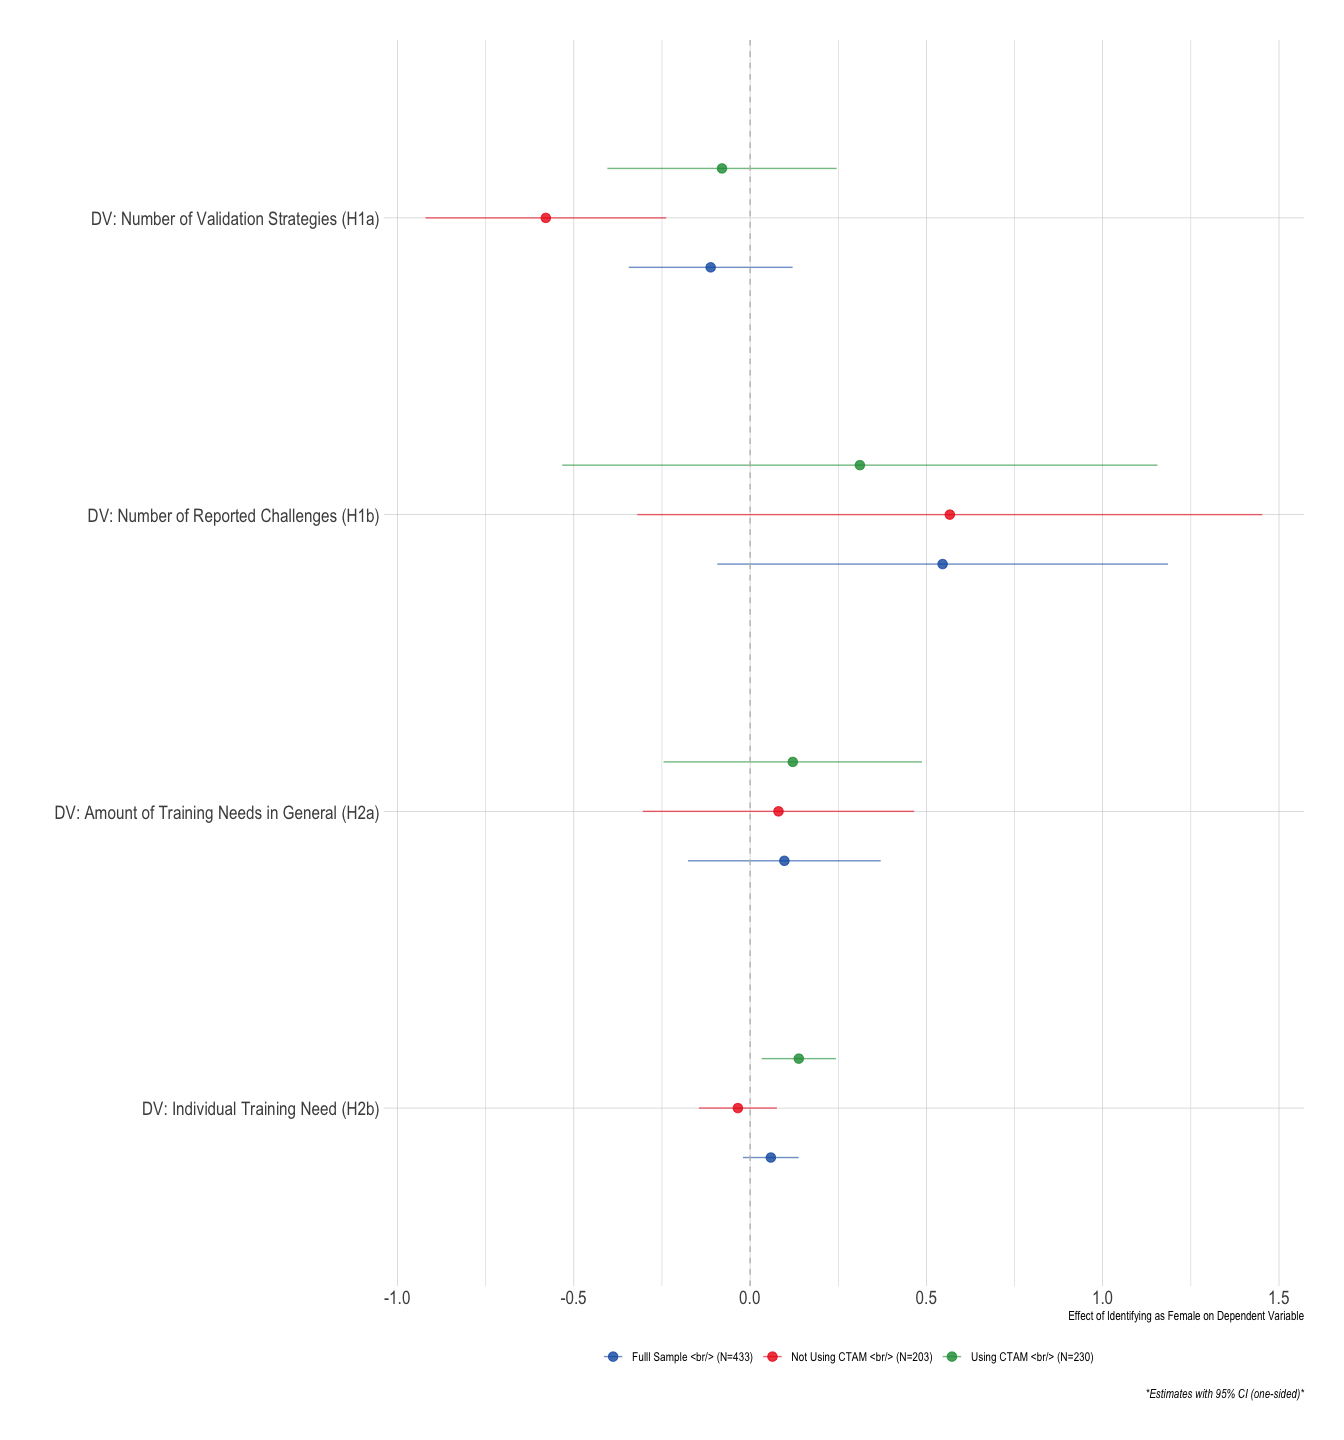
\includegraphics[width=0.9\textwidth,height=\textheight]{figures/h-pre-reg-1.png}

}

\caption{\label{fig:pre-reg-h}Effect of Being Female on Reported
Validation Strategies, Challenges, and Training Needs}

\end{figure}

Investigating the possible consequences of the Matilda effect further,
Figure \ref{fig:pre-reg-h} demonstrates that women scholars are also
more likely to report more training needs, but this effect is not
statistically significant. Looking at the type of training needs in the
bottom-left panel of Figure \ref{fig:dv-types}, we see that the
insignificance of the aggregated training needs stems from women using
CTAM and using manual content analysis reporting opposite needs: Women
in CTAM report general needs for training in research integrity and
ethics as well as for training in concepts, whereas women not using CTAM
report general training needs for programming and software skills as
well as for data and open access tools. Importantly, when it comes to
individual training needs, women scholars using CTAM do report they need
more training compared to men scholars using CTAM. This can serve as an
indication of consequences of the Matilda Effect at work, given that
research suggest that women are less likely to be invited on projects
(Evans and Moulder 2011; König and Ropers 2018). Using the data of Baden
et al. (2021), we see that women are less likely to be first author --
\texttt{47\%} of published papers on text analysis have an author with a
female first name. An independent \texttt{t-test} confirms that this
difference is statistically significant. The same holds for second and
third authors -- they are statistically significant more likely to be
male. This could lead to the perception that \emph{if one had more
training}, one would be asked to join projects too.

\begin{figure}[H]

{\centering 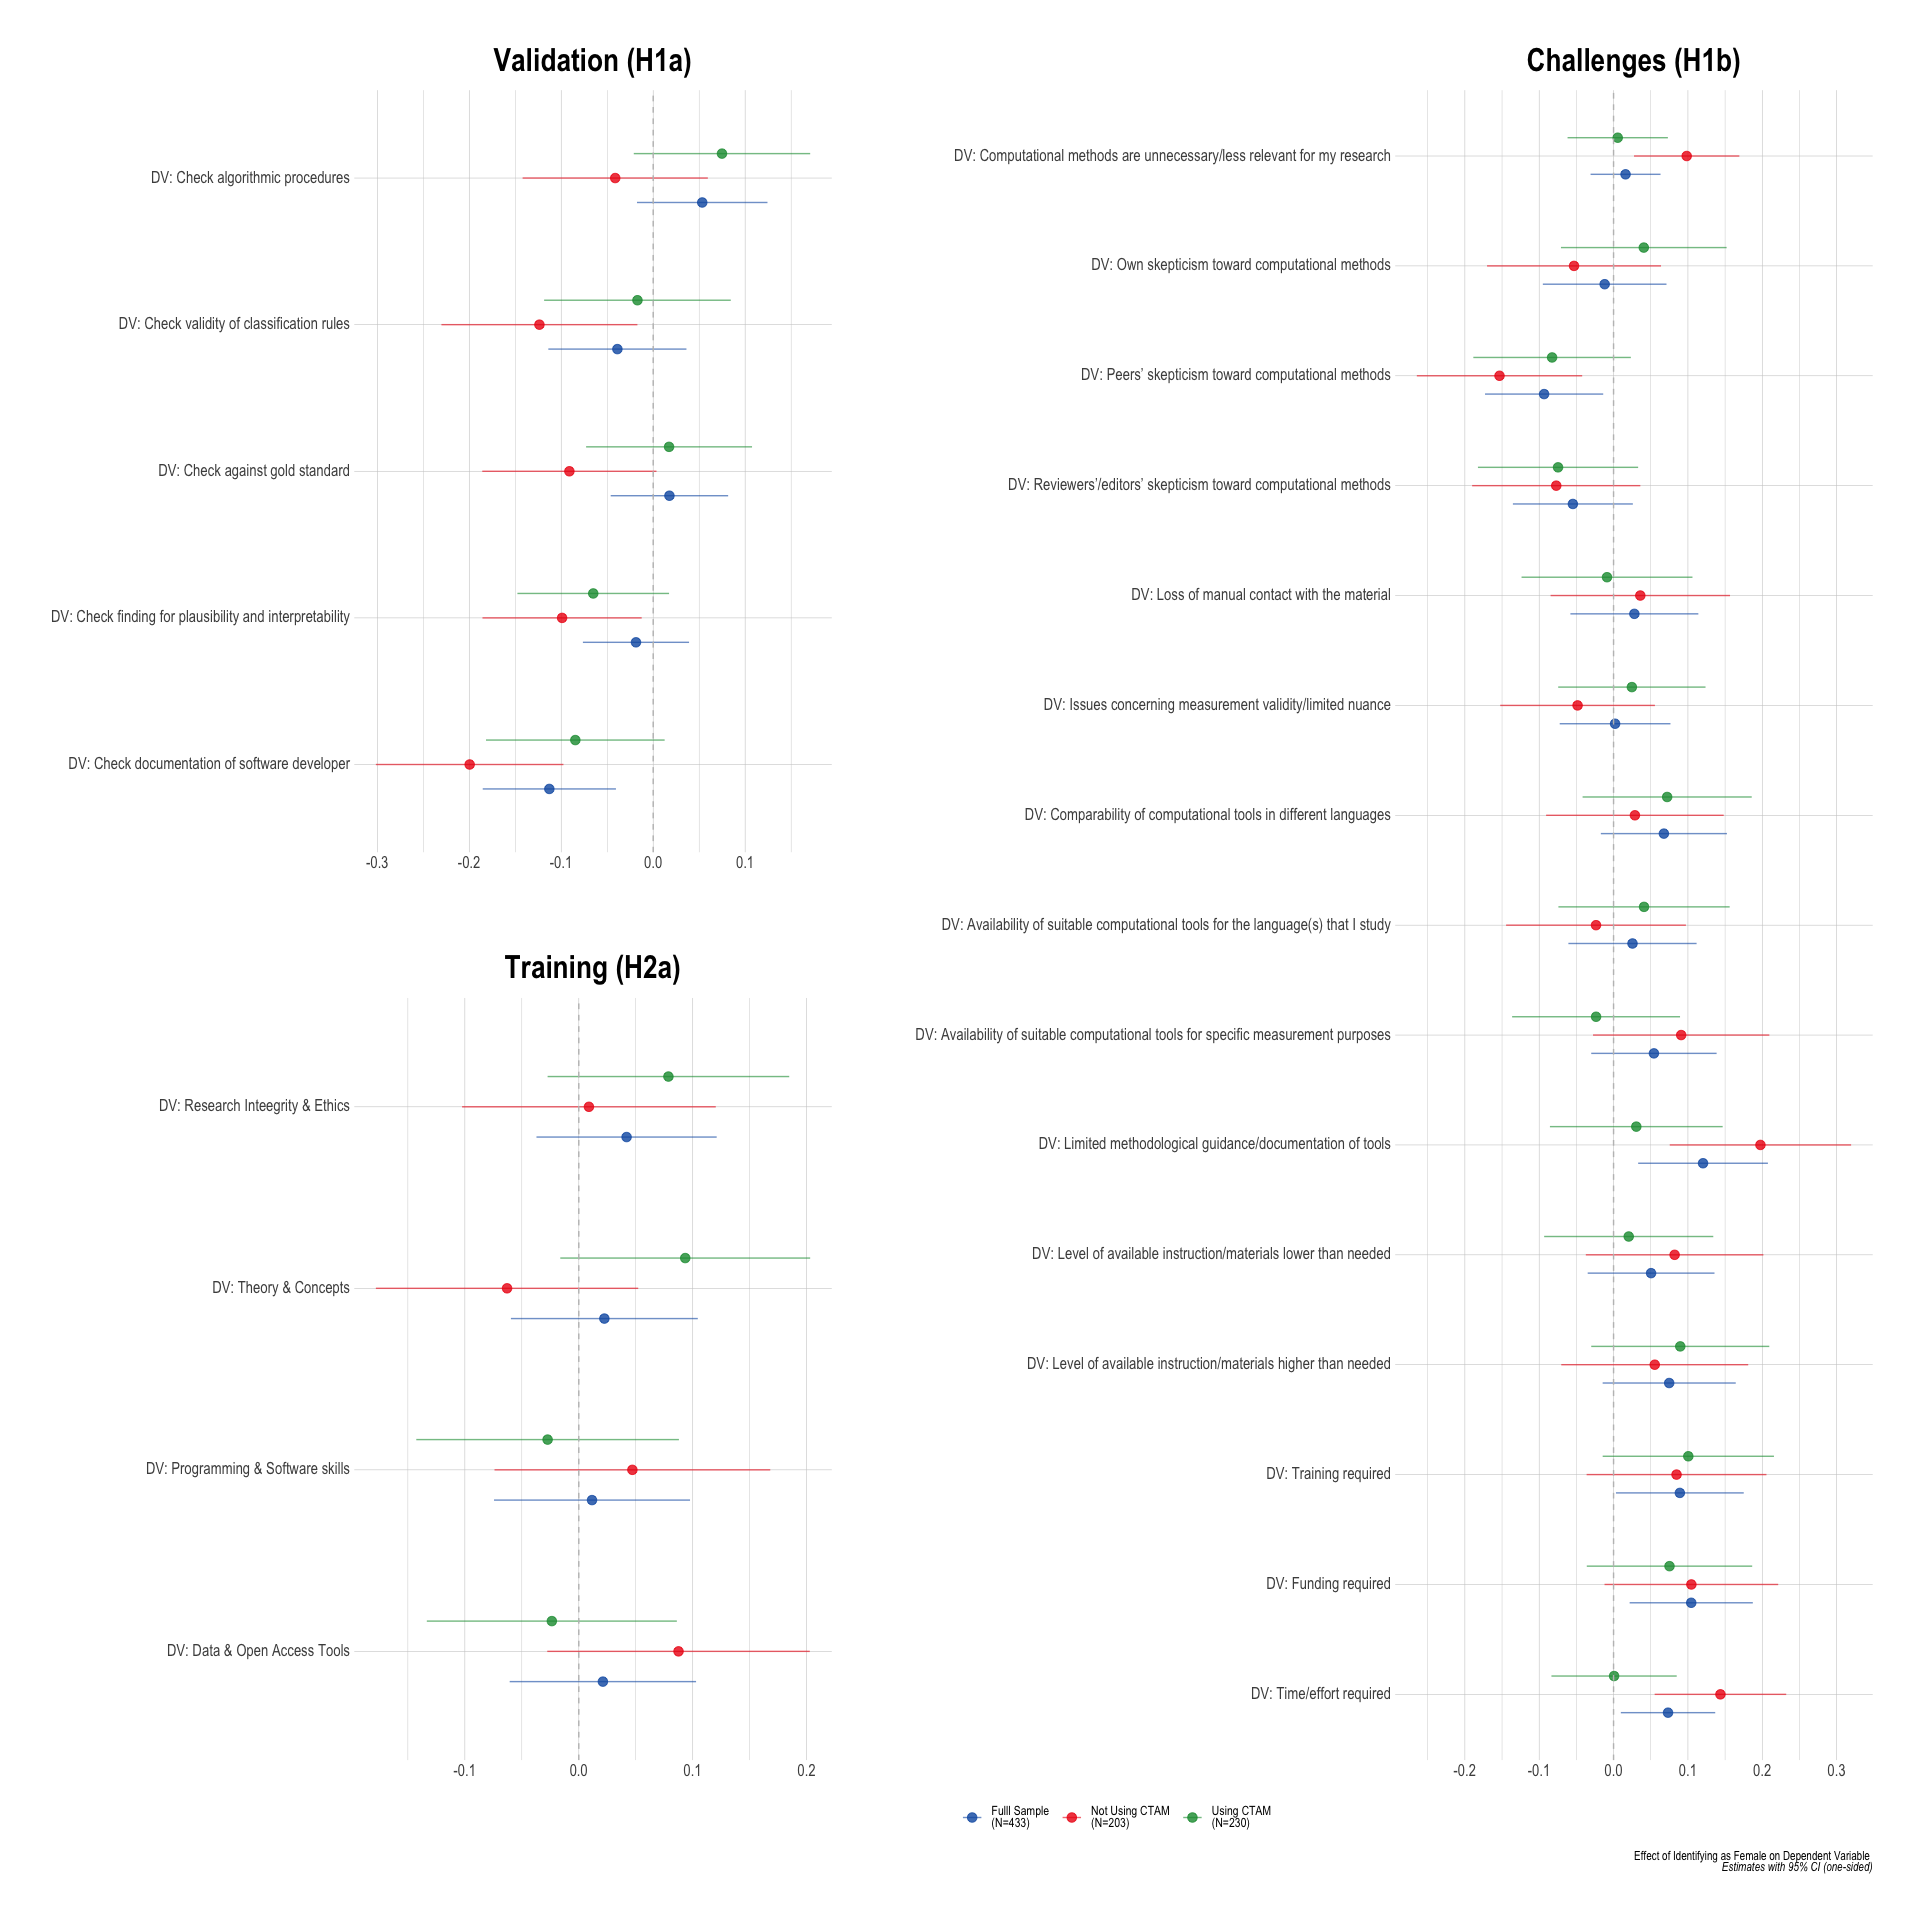
\includegraphics[width=1\textwidth,height=\textheight]{figures/types-dv-1.png}

}

\caption{\label{fig:dv-types}Effect of Being Female on Reported Type of
Validation Strategies, Challenges, and Training Needs}

\end{figure}

In addition to the pre-registered effects, we explored the interaction
with discipline and stage of the career of scholars, as demonstrated in
Figure \ref{fig:explor}. The left-hand panel of Figure \ref{fig:explor}
shows that compared to communication and political science, the other
disciplines (grouping sociology, psychology, and economy), where
computational methods were less common, we see support for both our
playing it safe and Matilda effect hypotheses. This can be
optimistically interpreted: When CTAM is more prevalent in the
discipline, women scholars catch up quickly. The right-hand panel of
Figure \ref{fig:explor} demonstrates that none of the reported results
are driven by a particular career stage of scholars.

\begin{figure}[H]

{\centering 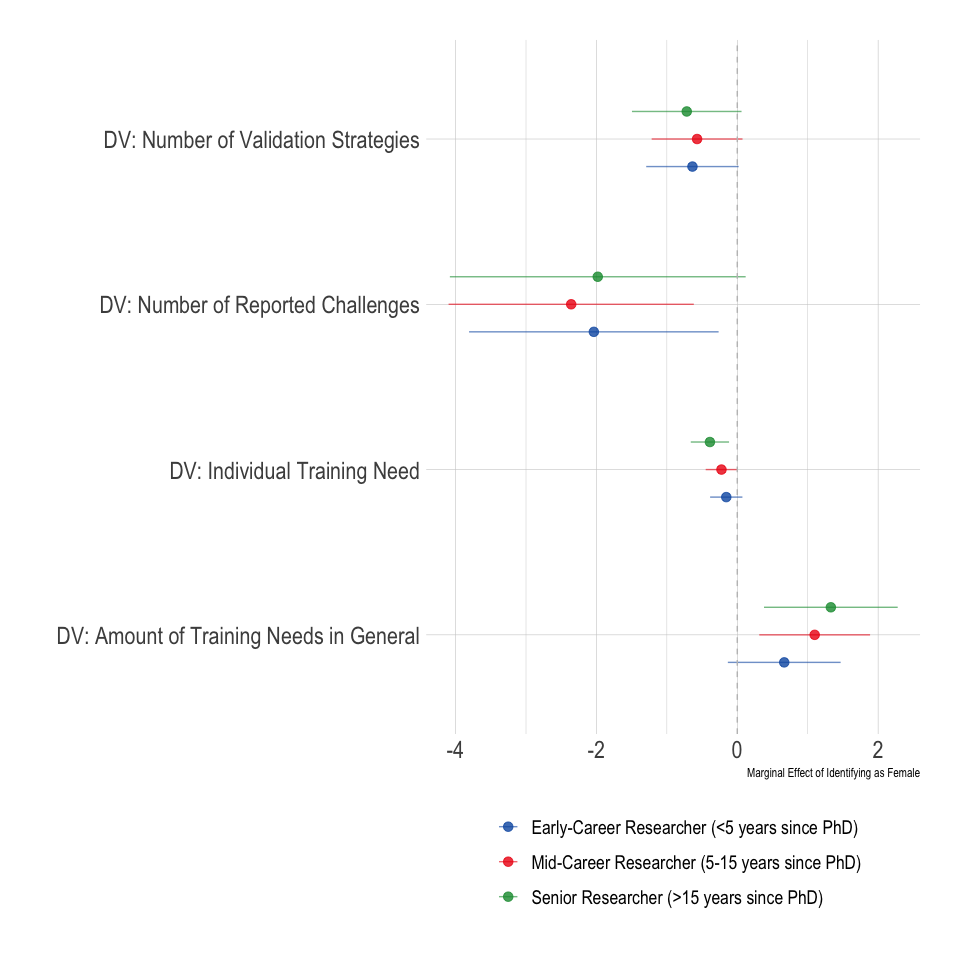
\includegraphics[width=1\textwidth,height=\textheight]{figures/explorative-2.png}

}

\caption{\label{fig:explor}Marginal Effect of Being Female on Reported
Validation Strategies, Challenges, and Training Needs}

\end{figure}

\hypertarget{discussion}{%
\section{Discussion}\label{discussion}}

This article presents an analysis of recently collected data from a
pre-registered expert survey of all authors of quantitative text
analytic research identified via a unique content analysis of research
articles published in the top 20 journals in communication science,
political science, sociology and psychology between 2016 and 2020
(\texttt{N\ =\ 854\ articles}). Using these data, our aim was to
understand whether and how using CTAM differs between men and women
scholars. According to the existing literature, gender gaps in methods
training and applications can have broader consequences for academic
careers. Examining authors' gender distribution among the 854 articles
using quantitative textual analysis shows a significant gender gap
especially in CTAM studies which were authored by 501 male scholars
compared to only 209 female scholars. These patterns underlay the
importance of an introspective evaluation of what might explain this
observed gender gap. Examining the survey data, we find that women are
more likely to report as major challenges to use of CTAM time/effort,
funding, and training needs and limited methodological guidance while
men are more concerned by peers' and editors' skepticism towards the
method. Furthermore, and especially when it comes to individual training
needs, women scholars using CTAM report they need more training compared
to men scholars using CTAM. We argue that these can serve as an
indication of the consequences of the Matilda Effect at work and support
our assumption for a gender submission gap. It is important to note that
we have conducted a very hard test: Women that have published on and are
engaged with text analyses methods. This group is a least-likely group
for whom gender disparities should occur, since they have supposedly
surpassed our assumption regarding a gendered submission gap - they have
published work using text analysis (both computational and manual). They
have thus also surpassed the expectation of discrimination which already
influences women's decision to submit manuscripts or not (König and
Ropers 2018) -- i.e.~these are women that have submitted and went
through the review-process are based on a particular self-selected
sample. It is therefore remarkable and telling that even in this curated
sample, we still find some indications for the fact that women have
internalized the Matilda effect and adapted their scientific practices
as such. That said, our findings our slightly optimistic: We show that
for the ``playing it safe'' strategy, there are no statistically
significant differences between men and women for the whole sample. When
we split the sample according to disciplines, we see that in the
disciplines where CTAM is more or less mainstream, the main conclusion
holds. In disciplines where this is not the case, women play it safe.
This aligns with Hill and Hurley (2022)'s finding that time in the
profession is crucial for publication gaps, albeit the fact that men
especially benefit from this cohort effect compared to women. Possible,
when CTAM is more embedded in the discipline, the gender imbalance is
not as apparent anymore. Men traditionally benefit more from
collaborations (e.g.~see Djupe, Smith, and Sokhey 2019), especially at
the early career stage which is arguably crucial in influencing
retention in the profession. We do not see that this relationship is
rank dependent, while rank is typically something that alleviates the
gender difference in the submission process (Brown and Samuels 2018).
That is great news, since the early career stage is arguably crucial in
influencing retention in the profession.

Looking deeper into how women play it safe, we see that women are more
likely to check if what they do computationally is in line with what the
program/algorithm says it does. However, they are less likely to check
``under the hood'' of the used program. In similar vein, the biggest
challenges for women not to use CTAM are a) the limited methodological
guidance and documentation of the software; and b) the time one has to
invest -- supposedly -- to learn these methods. This ties in with the
work on socialization into the profession: ``{[}D{]}ecisions about where
to submit, how often-and whether and where to submit\ldots{} tend to be
shaped by interpersonal contacts and information communicated through
social networks, as well as habits acquired through collaborative
relationships, which often differ by gender'' (Brown et al. 2020, 119).
Additionally, this finding about women's biggest challenges collides
with the Matilda Effect findings: Women report to be held back by things
that seem technical and therefore would cost them a lot of effort.

Our results do indicate the consequences of a Matilda effect at work:
Women report that there are in general enough training offered, but that
\emph{they} would need more training before up-taking these methods.
This could align with (perceived) success they have had publishing
papers using CTAM or just attempting to apply these methods. Previous
success creates both a sense of accomplishment and achievement that
fosters confidence in future success as well as leads to actual success,
since more publications result in a more successful career. If men
experience this more than women over time (the combined influence of the
Matthew and the Matilda effects), and men are at the heart of the
networks that socialize yet more men into the same perceptions and
attitudes, there perpetuates an environment that is ultimately more
supportive of the successful development of men's academic careers than
women's. That is, the under-recognition of women's work results, whether
purposefully or not, in the perception that a lot more effort is
required for women to succeed in the profession.

Our findings especially underline the persistence of the Matilda Effect
in academic work. The under-recognition of women in the sciences and the
social sciences (Rossiter 1993), endures across decades. Even if this is
mitigate in recent years, where women are more recognized vis-à-vis the
past, they are still unable to match the scholarly recognition men
receive for their work (Tatalovich and Frendreis 2019). It is therefore
of utmost importance that data and training infrastructure projects take
gender disparities, especially those coming from long gendered history
serious and accommodate alleviation strategies.

\newpage

\hypertarget{references}{%
\section*{References}\label{references}}
\addcontentsline{toc}{section}{References}

\hypertarget{refs}{}
\begin{CSLReferences}{1}{0}
\leavevmode\vadjust pre{\hypertarget{ref-alter_gender_2020}{}}%
Alter, Karen J., Jean Clipperton, Emily Schraudenbach, and Laura Rozier.
2020. {``Gender and {Status} in {American} {Political} {Science}: {Who}
{Determines} {Whether} a {Scholar} {Is} {Noteworthy}?''}
\emph{Perspectives on Politics} 18 (4): 1048--67.
\url{https://doi.org/10.1017/S1537592719004985}.

\leavevmode\vadjust pre{\hypertarget{ref-baden2021three}{}}%
Baden, Christian, Christian Pipal, Martijn Schoonvelde, and Mariken AC G
van der Velden. 2021. {``Three {Gaps} in {Computational} {Text}
{Analysis} {Methods} for {Social} {Sciences}: {A} {Research}
{Agenda}.''} \emph{Communication Methods and Measures}, 1--18.
\url{https://doi.org/10.1080/19312458.2021.2015574}.

\leavevmode\vadjust pre{\hypertarget{ref-barnes_2018}{}}%
Barnes, Tiffany D. 2018. {``Strategies for {Improving} {Gender}
{Diversity} in the {Methods} {Community}: {Insights} from {Political}
{Methodologists} and {Social} {Science} {Research}.''} \emph{PS:
Political Science and Politics} 51 (3): 580--87.
\url{https://doi.org/10.1017/S1049096518000513}.

\leavevmode\vadjust pre{\hypertarget{ref-barnes_beaulieu_2017}{}}%
Barnes, Tiffany D., and Emily Beaulieu. 2017. {``Engaging {Women}:
{Addressing} the {Gender} {Gap} in {Women}'s {Networking} and
{Productivity}.''} \emph{PS: Political Science and Politics} 50 (2):
461--66. \url{https://doi.org/10.1017/S1049096516003000}.

\leavevmode\vadjust pre{\hypertarget{ref-breuning_clearing_2018}{}}%
Breuning, Marijke, Benjamin Isaak Gross, Ayal Feinberg, Melissa
Martinez, Ramesh Sharma, and John Ishiyama. 2018. {``Clearing the
{Pipeline}? {Gender} and the {Review} {Process} at the {American}
{Political} {Science} {Review}.''} \emph{PS: Political Science and
Politics} 51 (3): 629--34.
\url{https://doi.org/10.1017/S1049096518000069}.

\leavevmode\vadjust pre{\hypertarget{ref-brown_horiuchi_htun_samuels_2020}{}}%
Brown, Nadia E., Yusaku Horiuchi, Mala Htun, and David Samuels. 2020.
{``Gender {Gaps} in {Perceptions} of {Political} {Science}
{Journals}.''} \emph{PS: Political Science and Politics} 53 (1):
114--21. \url{https://doi.org/10.1017/S1049096519001227}.

\leavevmode\vadjust pre{\hypertarget{ref-brown_samuels_2018}{}}%
Brown, Nadia E., and David Samuels. 2018. {``Beyond the {Gender}
{Citation} {Gap}: {Comments} on {Dion}, {Sumner}, and {Mitchell}.''}
\emph{Political Analysis} 26 (3): 328--30.
\url{https://doi.org/10.1017/pan.2018.14}.

\leavevmode\vadjust pre{\hypertarget{ref-cole_singer_1991}{}}%
Cole, Jonathan R., and Burton Singer. 1991. {``A {Theory} of {Limited}
{Differences}: {Explaining} the {Productivity} {Puzzle} in {Science}.''}
In \emph{The {Outer} {Circle}: {Women} in the {Scientific} {Community}},
edited by Jonathan R. Cole Harriet Zuckerman and John T. Bruer,
277--310. New York: Norton.

\leavevmode\vadjust pre{\hypertarget{ref-colgan_where_2016}{}}%
Colgan, Jeff D. 2016. {``Where {Is} {International} {Relations} {Going}?
{Evidence} from {Graduate} {Training}.''} \emph{International Studies
Quarterly} 60 (3): 486--98. \url{https://doi.org/10.1093/isq/sqv017}.

\leavevmode\vadjust pre{\hypertarget{ref-dion_sumner_mitchell_2018}{}}%
Dion, Michelle L., Jane Lawrence Sumner, and Sara McLaughlin Mitchell.
2018. {``Gendered {Citation} {Patterns} Across {Political} {Science} and
{Social} {Science} {Methodology} {Fields}.''} \emph{Political Analysis}
26 (3): 312--27. \url{https://doi.org/10.1017/pan.2018.12}.

\leavevmode\vadjust pre{\hypertarget{ref-djupe_smith_sokhey_2019}{}}%
Djupe, Paul A., Amy Erica Smith, and Anand Edward Sokhey. 2019.
{``Explaining {Gender} in the {Journals}: {How} {Submission} {Practices}
{Affect} {Publication} {Patterns} in {Political} {Science}.''} \emph{PS:
Political Science and Politics} 52 (1): 71--77.
\url{https://doi.org/10.1017/S104909651800104X}.

\leavevmode\vadjust pre{\hypertarget{ref-esarey_2018}{}}%
Esarey, Justin. 2018. {``What {Makes} {Someone} a {Political}
{Methodologist}?''} \emph{PS: Political Science and Politics} 51 (3):
588--96. \url{https://doi.org/10.1017/S1049096518000525}.

\leavevmode\vadjust pre{\hypertarget{ref-evans_moulder_2011}{}}%
Evans, Heather K., and A. Moulder. 2011. {``Reflecting on a {Decade} of
{Women}'s {Publications} in {Four} {Top} {Political} {Science}
{Journals}.''} \emph{PS: Political Science and Politics} 44 (4):
793--98.

\leavevmode\vadjust pre{\hypertarget{ref-ferber_gender_2011}{}}%
Ferber, Marianne A., and Michael Brün. 2011. {``The {Gender} {Gap} in
{Citations}: {Does} {It} {Persist}?''} \emph{Feminist Economics} 17 (1):
151--58. \url{https://doi.org/10.1080/13545701.2010.541857}.

\leavevmode\vadjust pre{\hypertarget{ref-gatto2020selecting}{}}%
Gatto, Malu AC, Anita R Gohdes, Denise Traber, and Mariken ACG Van Der
Velden. 2020. {``Selecting in or {Selecting} {Out}? {Gender} {Gaps} and
{Political} {Methodology} in {Europe}.''} \emph{PS: Political Science
and Politics} 53 (1): 122--27.
\url{https://doi.org/10.1017/S1049096519001288}.

\leavevmode\vadjust pre{\hypertarget{ref-gruber2023}{}}%
Gruber, Johannes B., and Mariken A. C. G. van der Velden. 2023.
{``Rethinking Software Documentation: Creating Inclusive Computational
Tools for Social Sciences.''}

\leavevmode\vadjust pre{\hypertarget{ref-hancock_women_2013}{}}%
Hancock, Kathleen J., Matthew A. Baum, and Marijke Breuning. 2013.
{``Women and {Pre}-{Tenure} {Scholarly} {Productivity} in
{International} {Studies}: {An} {Investigation} into the {Leaky}
{Career} {Pipeline}.''} \emph{International Studies Perspectives} 14
(4): 507--27.

\leavevmode\vadjust pre{\hypertarget{ref-hengel2017publishing}{}}%
Hengel, Erin. 2017. {``Publishing While {Female}. {Are} Women Held to
Higher Standards? {Evidence} from Peer Review.''}
\url{https://doi.org/10.17863/CAM.17548}.

\leavevmode\vadjust pre{\hypertarget{ref-hill_hurley_2022}{}}%
Hill, Kim Quaile, and Patricia A. Hurley. 2022. {``New {Evidence} on the
{Relative} {Scholarly} {Productivity} of {Male} Versus {Female}
{Political} {Scientists}.''} \emph{PS: Political Science and Politics}
55 (4): 788--92. \url{https://doi.org/10.1017/S1049096522000683}.

\leavevmode\vadjust pre{\hypertarget{ref-Huang_et_al_2020}{}}%
Huang, Junming, Alexander J. Gates, Roberta Sinatra, and Albert-László
Barabási. 2020. {``Historical Comparison of Gender Inequality in
Scientific Careers Across Countries and Disciplines.''}
\emph{Proceedings of the National Academy of Sciences} 117 (9):
4609--16. \url{https://doi.org/10.1073/pnas.1914221117}.

\leavevmode\vadjust pre{\hypertarget{ref-key_sumner_2019}{}}%
Key, Ellen M., and Jane Lawrence Sumner. 2019. {``You {Research} {Like}
a {Girl}: {Gendered} {Research} {Agendas} and {Their} {Implications}.''}
\emph{PS: Political Science and Politics} 52 (4): 663--68.
\url{https://doi.org/10.1017/S1049096519000945}.

\leavevmode\vadjust pre{\hypertarget{ref-kim_grofman_2019}{}}%
Kim, Hanna June, and Bernard Grofman. 2019. {``Job {Mobility}, {Tenure},
and {Promotions} in {Political} {Science} {PhD}-{Granting}
{Departments}, 2002--2017: {Cohort}, {Gender}, and {Citation}-{Count}
{Effects}.''} \emph{PS: Political Science and Politics} 52 (4): 684--90.
\url{https://doi.org/10.1017/S1049096519000490}.

\leavevmode\vadjust pre{\hypertarget{ref-knobloch-westerwick_matilda_2013}{}}%
Knobloch-Westerwick, Silvia, and Carroll J. Glynn. 2013. {``The
{Matilda} {Effect}---{Role} {Congruity} {Effects} on {Scholarly}
{Communication}: {A} {Citation} {Analysis} of {Communication} {Research}
and {Journal} of {Communication} {Articles}.''} \emph{Communication
Research} 40 (1): 3--26. \url{https://doi.org/10.1177/0093650211418339}.

\leavevmode\vadjust pre{\hypertarget{ref-konig_ropers_2018}{}}%
König, Thomas, and Guido Ropers. 2018. {``Gender and {Editorial}
{Outcomes} at the {American} {Political} {Science} {Review}.''}
\emph{PS: Political Science and Politics} 51 (4): 849--53.
\url{https://doi.org/10.1017/S1049096518000604}.

\leavevmode\vadjust pre{\hypertarget{ref-krippendorff2013}{}}%
Krippendorff, Klaus. 2013. \emph{Content {Analysis}: {An} {Introduction}
to {Its} {Methodology}}. SAGE.

\leavevmode\vadjust pre{\hypertarget{ref-lazer2020computational}{}}%
Lazer, David MJ, Alex Pentland, Duncan J Watts, Sinan Aral, Susan Athey,
Noshir Contractor, Deen Freelon, et al. 2020. {``Computational Social
Science: {Obstacles} and Opportunities.''} \emph{Science} 369 (6507):
1060--62.

\leavevmode\vadjust pre{\hypertarget{ref-ma_etal_2019}{}}%
Ma, Yifang, Diego F. M. Oliveira, Teresa K. Woodruff, and Brian Uzzi.
2019. {``Women Who Win Prizes Get Less Money and Prestige.''}
\emph{Nature} 565 (7739): 287--88.
\url{https://doi.org/10.1038/d41586-019-00091-3}.

\leavevmode\vadjust pre{\hypertarget{ref-macnell_2015}{}}%
MacNell, Lillian, Adam Driscoll, and Andrea N. Hunt. 2015. {``What's in
a {Name}: {Exposing} {Gender} {Bias} in {Student} {Ratings} of
{Teaching}.''} \emph{Innovative Higher Education} 40: 291--303.
\url{https://doi.org/10.1007/s10755-014-9313-4}.

\leavevmode\vadjust pre{\hypertarget{ref-Madera_et_al_2019}{}}%
Madera, Juan M., Michelle R. Hebl, Heather Dial, Randi Martin, and
Virgina Valian. 2019. {``Raising {Doubt} in {Letters} of
{Recommendation} for {Academia}: {Gender} {Differences} and {Their}
{Impact}.''} \emph{Journal of Business and Psychology} 34: 287--303.
\url{https://doi.org/10.1007/s10869-018-9541-1}.

\leavevmode\vadjust pre{\hypertarget{ref-maliniak_etal_2008}{}}%
Maliniak, Daniel, Amy Oakes, Susan Peterson, and Michael J. Tierney.
2008. {``Women in {International} {Relations}.''} \emph{Politics and
Gender} 4 (1): 122--44. \url{https://doi.org/10.1017/S1743923X08000068}.

\leavevmode\vadjust pre{\hypertarget{ref-maliniak_powers_walter_2013}{}}%
Maliniak, Daniel, Ryan Powers, and Barbara F. Walter. 2013. {``The
{Gender} {Citation} {Gap} in {International} {Relations}.''}
\emph{International Organization} 67 (4): 889--922.
\url{https://doi.org/10.1017/S0020818313000209}.

\leavevmode\vadjust pre{\hypertarget{ref-Mengel_et_al_2018}{}}%
Mengel, Friederike, Jan Sauermann, and Ulf Zölitz. 2018. {``Gender
{Bias} in {Teaching} {Evaluations}.''} \emph{Journal of the European
Economic Association} 17 (2): 535--66.
\url{https://doi.org/10.1093/jeea/jvx057}.

\leavevmode\vadjust pre{\hypertarget{ref-monroe_etal_2008}{}}%
Monroe, Kristen, Saba Ozyurt, Ted Wrigley, and Amy Alexander. 2008.
{``Gender {Equality} in {Academia}: {Bad} {News} from the {Trenches},
and {Some} {Possible} {Solutions}.''} \emph{Perspectives on Politics} 6
(2): 215--33. \url{https://doi.org/10.1017/S1537592708080572}.

\leavevmode\vadjust pre{\hypertarget{ref-morrow_box_2014}{}}%
Morrow-Jones, Hazel, and Janet M. Box-Steffensmeier. 2014. {``Implicit
{Bias} and {Why} {It} {Matters} to the {Field} of {Political}
{Methodology}.''} \emph{The Political Methodologist} 21 (2): 16--19.

\leavevmode\vadjust pre{\hypertarget{ref-oliveira_etal_2019}{}}%
Oliveira, Diego F. M., Yifang Ma, Teresa K. Woodruff, and Brian Uzzi.
2019. {``Comparison of {National} {Institutes} of {Health} {Grant}
{Amounts} to {First}-{Time} {Male} and {Female} {Principal}
{Investigators}.''} \emph{JAMA} 321 (9): 898--900.
\url{https://doi.org/10.1001/jama.2018.21944}.

\leavevmode\vadjust pre{\hypertarget{ref-phull_gender_2019}{}}%
Phull, Kiran, Gokhan Ciflikli, and Gustav Meibauer. 2019. {``Gender and
Bias in the {International} {Relations} Curriculum: {Insights} from
Reading Lists.''} \emph{European Journal of International Relations} 25
(2): 383--407. \url{https://doi.org/10.1177/1354066118791690}.

\leavevmode\vadjust pre{\hypertarget{ref-rossiter1993matthew}{}}%
Rossiter, Margaret W. 1993. {``The {Matthew} {Matilda} Effect in
Science.''} \emph{Social Studies of Science} 23 (2): 325--41.
\url{https://doi.org/10.1177/030631293023002004}.

\leavevmode\vadjust pre{\hypertarget{ref-salganik2019bit}{}}%
Salganik, Matthew J. 2019. \emph{Bit by Bit: {Social} Research in the
Digital Age}. Princeton University Press.

\leavevmode\vadjust pre{\hypertarget{ref-samuels_teele_2021}{}}%
Samuels, David J., and Dawn Langan Teele. 2021. {``New {Medium}, {Same}
{Story}? {Gender} {Gaps} in {Book} {Publishing}.''} \emph{PS: Political
Science and Politics} 54 (1): 131--40.
\url{https://doi.org/10.1017/S1049096520001018}.

\leavevmode\vadjust pre{\hypertarget{ref-sarkees_breuning_2010}{}}%
Sarkees, Meredith Reid, and Marijke Breuning. 2010. {``Incorporating
{Women} into {International} {Studies}: {Working} {Their} {Way} {In}.''}
In \emph{The {International} {Studies} {Encyclopedia}, a Component of
the {International} {Studies} {Compendium} {Project}}, edited by Robert
A Denemark and Renée Marlin-Bennet, 3640--56. UK: Wiley-Blackwell.

\leavevmode\vadjust pre{\hypertarget{ref-shannon2014barriers}{}}%
Shannon, Megan. 2014. {``Barriers to {Women}'s {Participation} in
{Political} {Methodology}: {Graduate} {School} and {Beyond}.''}
\emph{The Political Methodologist} 21 (2): 2--6.

\leavevmode\vadjust pre{\hypertarget{ref-tatalovich_frendries_2019}{}}%
Tatalovich, Raymond, and John Frendreis. 2019. {``Winning Awards and
Gaining Recognition: {An} Impact Analysis of {APSA} Section Book
Prizes.''} \emph{The Social Science Journal} 56: 316--23.
\url{https://doi.org/10.1016/j.soscij.2018.07.006}.

\leavevmode\vadjust pre{\hypertarget{ref-teele_thelen_2017}{}}%
Teele, Dawn Langan, and Kathleen Thelen. 2017. {``Gender in the
{Journals}: {Publication} {Patterns} in {Political} {Science}.''}
\emph{PS: Political Science and Politics} 50 (2): 433--47.
\url{https://doi.org/10.1017/S1049096516002985}.

\leavevmode\vadjust pre{\hypertarget{ref-Weisshaar_2017}{}}%
Weisshaar, Katherine. 2017. {``Publish and {Perish}? {An} {Assessment}
of {Gender} {Gaps} in {Promotion} to {Tenure} in {Academia}.''}
\emph{Social Forces} 96 (2): 529--60.
\url{https://doi.org/10.1093/sf/sox052}.

\leavevmode\vadjust pre{\hypertarget{ref-Welborn_McKenzie_1989}{}}%
Welborn, Tracey, and Danny L. McKenzie. 1989. {``{SCIENCE}
{ACHIEVEMENT}, {ATTITUDES} {AND} {CAREER} {SELECTION} {OF} {FEMALES}:
{A} {REVIEW} {OF} {RESEARCH}.''} \emph{Journal of Elementary Science
Education} 1 (2): 3--9. \url{https://doi.org/10.2307/43155578}.

\leavevmode\vadjust pre{\hypertarget{ref-Young_1995}{}}%
Young, Cheryl D. 1995. {``An {Assessment} of {Articles} {Published} by
{Women} in 15 {Top} {Political} {Science} {Journals}.''} \emph{PS:
Political Science and Politics} 28 (3): 525--33.
\url{https://doi.org/10.2307/420325}.

\end{CSLReferences}



\end{document}
